\documentclass[
	% -- opções da classe memoir --
	12pt,				% tamanho da fonte
	openright,			% capítulos começam em pág ímpar (insere página vazia caso preciso)
	twoside,			% para impressão em recto e verso. Oposto a oneside
	a4paper,			% tamanho do papel. 
	% -- opções da classe abntex2 --
	%chapter=TITLE,		% títulos de capítulos convertidos em letras maiúsculas
	%section=TITLE,		% títulos de seções convertidos em letras maiúsculas
	%subsection=TITLE,	% títulos de subseções convertidos em letras maiúsculas
	%subsubsection=TITLE,% títulos de subsubseções convertidos em letras maiúsculas
	% -- opções do pacote babel --
	english,			% idioma adicional para hifenização
	brazil				% o último idioma é o principal do documento
	]{abntex2}

% Pacotes básicos 
\usepackage{lmodern}			% Usa a fonte Latin Modern			
\usepackage[T1]{fontenc}		% Selecao de codigos de fonte.
\usepackage[utf8]{inputenc}		% Codificacao do documento (conversão automática dos acentos)
\usepackage{indentfirst}		% Indenta o primeiro parágrafo de cada seção.
\usepackage{color}				% Controle das cores
\usepackage{graphicx}			% Inclusão de gráficos
\usepackage{microtype} 			% para melhorias de justificação

% Pacote de glossario
\usepackage{./9_Extras/styles/anbtex2-glossario}

% Pacotes de citações
\usepackage[brazilian,hyperpageref]{backref}	 % Paginas com as citações na bibl
\usepackage[alf,abnt-emphasize=bf]{abntex2cite}	% Citações padrão ABNT
\input{./9_Extras/packagesConfig/backref}

% Pacotes para algoritmos
\usepackage{listings}
\renewcommand{\lstlistlistingname}{Lista de códigos-fonte} 
\renewcommand{\lstlistingname}{Código-fonte} 
\newlistof{lstlistoflistings}{lol}{\lstlistlistingname}

% Configuracoes gerais
%\lstset{ 
%  backgroundcolor=\color{white},   % choose the background color; you must add \usepackage{color} or \usepackage{xcolor}; should come as last argument
%  basicstyle=\footnotesize,        % the size of the fonts that are used for the code
%  breakatwhitespace=false,         % sets if automatic breaks should only happen at whitespace
%  breaklines=true,                 % sets automatic line breaking
%  captionpos=b,                    % sets the caption-position to bottom
%  commentstyle=\color{mygreen},    % comment style
%  deletekeywords={...},            % if you want to delete keywords from the given language
%  escapeinside={\%*}{*)},          % if you want to add LaTeX within your code
%  extendedchars=true,              % lets you use non-ASCII characters; for 8-bits encodings only, does not work with UTF-8
%  firstnumber=1000,                % start line enumeration with line 1000
%  frame=single,	                   % adds a frame around the code
%  keepspaces=true,                 % keeps spaces in text, useful for keeping indentation of code (possibly needs columns=flexible)
%  keywordstyle=\color{blue},       % keyword style
%  morekeywords={*,...},            % if you want to add more keywords to the set
%  numbers=left,                    % where to put the line-numbers; possible values are (none, left, right)
%  numbersep=5pt,                   % how far the line-numbers are from the code
%  numberstyle=\tiny\color{mygray}, % the style that is used for the line-numbers
%  rulecolor=\color{black},         % if not set, the frame-color may be changed on line-breaks within not-black text (e.g. comments (green here))
%  showspaces=false,                % show spaces everywhere adding particular underscores; it overrides 'showstringspaces'
%  showstringspaces=false,          % underline spaces within strings only
%  showtabs=false,                  % show tabs within strings adding particular underscores
%  stepnumber=2,                    % the step between two line-numbers. If it's 1, each line will be numbered
%  stringstyle=\color{mymauve},     % string literal style
%  tabsize=2,	                   % sets default tabsize to 2 spaces
%  title=\lstname                   % show the filename of files included with \lstinputlisting; also try caption instead of title
%}

\definecolor{listings_keyword}{RGB}{30,80,179}
\definecolor{listings_comment}{RGB}{82,151,82}
\definecolor{listings_identifier}{RGB}{0,0,0}
\definecolor{listings_string}{RGB}{225,89,89}
\definecolor{listings_emphs}{RGB}{159,77,153}
\lstset{
  belowcaptionskip=1\baselineskip,
  breaklines=true,
  frame=tbL,
  showstringspaces=false,
  basicstyle=\footnotesize\ttfamily,
  keywordstyle=\bfseries\color{listings_keyword},
  commentstyle=\itshape\color{listings_comment},
  identifierstyle=\color{listings_identifier},
  emphstyle=\color{listings_emphs},
  stringstyle=\color{listings_string},
  captionpos=b,
  escapechar=\§,
}

% Ajustes para linguagem Python
\lstdefinestyle{Python_lang}{
  language=Python,
  morekeywords={as},
  emph={import,return},
}


\usepackage{amsmath, amssymb}
% \usepackage{pgf}
\usepackage{pdfpages}

% Pacote para fracoes diagonais
\usepackage{xfrac}

% Cria comando para referência de anexos. https://github.com/abntex/abntex2/issues/76
\newcommand{\crefanexo}[1]{\hyperref[#1]{anexo~\ref{#1}}}
\newcommand{\Crefanexo}[1]{\hyperref[#1]{Anexo~\ref{#1}}}

% CONFIGURAÇÕES DE PACOTES

% Informações de dados para CAPA e FOLHA DE ROSTO
\titulo{Controle Preditivo Baseado em Modelo (MPC) aplicado a uma planta didática}
\autor{Tiago Correa Prata}
\local{São Paulo}
\data{2019}
\orientador{Alexandre Brincalepe Campo}
%\coorientador{----}
\instituicao{Instituto Federal de São Paulo - IFSP}
\tipotrabalho{Tese (Mestrado)}
% O preambulo deve conter o tipo do trabalho, o objetivo, 
% o nome da instituição e a área de concentração 
\preambulo{Projeto de pesquisa apresentado ao Instituto Federal de Educação, Ciência
e Tecnologia de São Paulo para a qualificação no programa de mestrado em engenharia
de automação e controle.}


% informações do PDF
\definecolor{PDF_blue}{RGB}{28,3,126}
\makeatletter
\hypersetup{
     	%pagebackref=true,
		pdftitle={\@title}, 
		pdfauthor={\@author},
    	pdfsubject={\imprimirpreambulo},
	    pdfcreator={LaTeX},
		pdfkeywords={MPC}{Model Predictive Control}{Controle Avançado}, 
		colorlinks=true,       		% false: boxed links; true: colored links
    	linkcolor=PDF_blue,          	% color of internal links
    	citecolor=PDF_blue,        		% color of links to bibliography
    	filecolor=magenta,      		% color of file links
		urlcolor=PDF_blue,
		bookmarksdepth=4
}
\makeatother

\usepackage[nameinlink, brazilian]{cleveref}

% Posiciona figuras e tabelas no topo da página quando adicionadas sozinhas
% em um página em branco.
\makeatletter
\setlength{\@fptop}{5pt} % Set distance from top of page to first float
\makeatother

% Possibilita criação de Quadros e Lista de quadros.
\newcommand{\quadroname}{Quadro}
\newcommand{\listofquadrosname}{Lista de quadros}

\newfloat[chapter]{quadro}{loq}{\quadroname}
\newlistof{listofquadros}{loq}{\listofquadrosname}
\newlistentry{quadro}{loq}{0}

% configurações para atender às regras da ABNT
\setfloatadjustment{quadro}{\centering}
\counterwithout{quadro}{chapter}
\renewcommand{\cftquadroname}{\quadroname\space} 
\renewcommand*{\cftquadroaftersnum}{\hfill--\hfill}

\setfloatlocations{quadro}{hbtp}

% Espaçamentos entre linhas e parágrafos 

% O tamanho do parágrafo é dado por:
\setlength{\parindent}{1.3cm}

% Controle do espaçamento entre um parágrafo e outro:
\setlength{\parskip}{0.2cm}  % tente também \onelineskip

% compila o indice
\makeindex

% GLOSSARIO
\makeglossaries

\input{./1_preText/glossarioItens}

% Exemplo de configurações do glossairo
\renewcommand*{\glsseeformat}[3][\seename]{\textit{#1}  
\glsseelist{#2}}

% ----------------------------------------------------------
% Início do documento
\begin{document}

% Seleciona o idioma do documento (conforme pacotes do babel)
%\selectlanguage{english}
\selectlanguage{brazil}

% Retira espaço extra obsoleto entre as frases.
\frenchspacing 

% ELEMENTOS PRÉ-TEXTUAIS
% \pretextual

% Capa
\imprimircapa

% Folha de rosto
% (o * indica que haverá a ficha bibliográfica)
\imprimirfolhaderosto
% \imprimirfolhaderosto*	% TODO: Substituir por essa linha quando inserir Ficha Catalografica

% Inserir a ficha bibliografica
%\include{./1_pretext/fichaCatalografica}

% Inserir errata
%\include{./1_pretext/errata}

% Inserir folha de aprovação
% Isto é um exemplo de Folha de aprovação, elemento obrigatório da NBR
% 14724/2011 (seção 4.2.1.3). Você pode utilizar este modelo até a aprovação
% do trabalho. Após isso, substitua todo o conteúdo deste arquivo por uma
% imagem da página assinada pela banca com o comando abaixo:
%
% \begin{folhadeaprovacao}
% \includepdf{folhadeaprovacao_final.pdf}
% \end{folhadeaprovacao}
%
\begin{folhadeaprovacao}

  \begin{center}
    {\ABNTEXchapterfont\large\imprimirautor}

    \vspace*{\fill}\vspace*{\fill}
    \begin{center}
      \ABNTEXchapterfont\bfseries\Large\imprimirtitulo
    \end{center}
    \vspace*{\fill}
    
    \hspace{.45\textwidth}
    \begin{minipage}{.5\textwidth}
        \imprimirpreambulo
    \end{minipage}%
    \vspace*{\fill}
   \end{center}
        
   Trabalho aprovado. \imprimirlocal, 20 de agosto de 2020:

   \assinatura{\textbf{\imprimirorientador} \\ Orientador} 
   \assinatura{\textbf{Prof. Dr. Eduardo Alves da Costa} \\ Convidado (interno)}
   \assinatura{\textbf{Prof. Dr. Diego Colón} \\ Convidado (externo)}
   \assinatura{\textbf{Prof. Dr. Ricardo Pires} \\ Suplente (interno)}
   \assinatura{\textbf{Prof. Dr. Wânderson de Oliveira Assis} \\ Suplente (externo)}
      
   \begin{center}
    \vspace*{0.5cm}
    {\large\imprimirlocal}
    \par
    {\large\imprimirdata}
    \vspace*{1cm}
  \end{center}
  
\end{folhadeaprovacao}

% Dedicatória
%\begin{dedicatoria}
   \vspace*{\fill}
   \centering
   \noindent
   \textit{ Texto da dedicatória } \vspace*{\fill}
\end{dedicatoria}

% Agradecimentos
%\begin{agradecimentos}

Os agradecimentos principais são direcionados aos meus pais Aurimar e Jair,
por proporcionarem aos filhos o privilégio de poderem estudar sem que nada jamais
faltasse; à minha irmã Thais, que apesar dos milhares de quilômetros de distância
seu carinho e incentivo para a conclusão desse trabalho nunca cessaram; e a minha
companheira Evelyn, pelo apoio e dedicação durante essa trajetória e por compartilhar
comigo a experiência de passar por um mestrado. Amo vocês!

Agradecimentos especiais direcionados ao meu orientador Dr. Alexandre Brincalepe Campo
que apesar da intensa rotina de sua vida acadêmica aceitou me orientar e me fez indicações
valiosas que fizeram toda a diferença; e ao Instituto Federal de Educação, Ciência e
Tecnologia de São Paulo, essencial no meu processo de formação profissional.

\end{agradecimentos}

% Epígrafe
%\include{./1_pretext/epigrafe}


% RESUMOS

% resumo em português
\setlength{\absparsep}{18pt} % ajusta o espaçamento dos parágrafos do resumo
\begin{resumo}
    % TODO: Fazer resumo
    
    \vspace{\onelineskip}

    \noindent 
    \textbf{Palavras-chave}: 
\end{resumo}

% resumo em inglês
\setlength{\absparsep}{18pt} % ajusta o espaçamento dos parágrafos do resumo
\begin{resumo}[Abstract]
  \begin{otherlanguage*}{english}
    \acrshort{mpc} is a control technique that has been gaining attention and refinement over the last 50 years
    and it is currently one of the most prominent techniques in predictive control, having numerous
    commercial applications since its implementation in multivariate chemical process control,
    to the construction of logics for the orientation of autonomous vehicles.
    
    This dissertation deals with the development of a model based predictive control, applied
    to a pilot plant, addressing the whole process of construction and development of it,
    aiming to provide a clear understanding of each of the stages.
    
    This project can be divided into 6 different parts: basic theory of predictive control;
    theories about \acrshort{mpc}; systems identification; construction of the predictive controller;
    application and analysis. The whole practical part of this project is developed in \acrshort{matlab}
    and/or \textit{Python}, and implemented in an easily accessible educational plan, aiming for
    easy replicability.

    \vspace{\onelineskip}

    \noindent 
    \textbf{Keywords}: model predictive control; predictive contro; control theory; system identification
  \end{otherlanguage*}
\end{resumo}

% inserir lista de ilustrações
\pdfbookmark[0]{\listfigurename}{lof}
\listoffigures*
\cleardoublepage

% TODO: Reinserir lista de quadros quando houverem quadros
% % inserir lista de quadros
% \pdfbookmark[0]{\listofquadrosname}{loq}
% \listofquadros*
% \cleardoublepage

% % inserir lista de tabelas
\pdfbookmark[0]{\listtablename}{lot} 
\listoftables*
\cleardoublepage

% inserir lista de algoritmos
\pdfbookmark[0]{\lstlistlistingname}{lol}
\lstlistoflistings*
\cleardoublepage

% inserir lista de abreviaturas e siglas
\imprimirlistadesiglas

% inserir lista de símbolos
\imprimirlistadesimbolos 
\setcounter{table}{0}	% Comando inserido para ajustar numeracao de tabelas

% inserir o sumario
\pdfbookmark[0]{\contentsname}{toc}
\tableofcontents*
\cleardoublepage


% ELEMENTOS TEXTUAIS
\textual

% PARTE APRESENTACAO
\part{Apresentação}

\newacronym{mimo}{MIMO}{Multiple Input Multiple Output}
\newacronym{pid}{PID}{Proporcional Integral Derivativo}
\newacronym{mpc}{MPC}{Model Predictive Control}
\chapter{Introdução}

%Controle de processos é fundamental na industria.	[ok]
%Objetivo do controle.								[ok]
%Otimizar além de controlar.						[ok]
%Estratégias utilizando modelos matemáticos.		[ok]
%Porque não usar PID em alguns casos?				[ok - mais ou menos]
%Conceito do MPC.									[ok]
O controle de processos tem fundamental importância no desenvolvimento industrial, sendo amplamente utilizado em praticamente todos os segmentos da indústria, contribuindo de maneira significativa para a maior velocidade na estabilização de sinais, aumento da qualidade de produtos, diminuição de riscos e redução de custos operacionais. Seu objetivo, de forma simplificada, consiste em avaliar e corrigir desvios entre um valor desejado e o real valor medido na saída da planta para uma dada variável do processo (ou variáveis, como em casos de processos com multiplas entradas e multiplas saídas, também conhecidos por sua sigla em inglês \acrshort{mimo} (\textit{\acrlong{mimo}})). A aplicação correta de estratégias de controle acarreta numa operação eficiênte da planta, mantendo suas variáveis relevantes em condições próximas as desejadas. A sintonia bem feita do controle auxilia também na otimização do processo, possibilitando que o sistema opere com menor variabilidade, maximizando a produção e minimizando a utilização de recursos. No \autoref{otimizacao} abordaremos mais sobre otimização.
Modelos matemáticos podem auxiliar a estratégia de controle uma vez que um modelo da planta ou processo pode ser utilizado para estabelecer a relação existente entre as variáveis manipuladas e variáveis controladas, assim podendo auxiliar na predição do comportamento dinâmico do sistema analisado. A modelagem matemática pode ser feita utilizando dados empíricos ou através da aplicação de relações físico-químicas.

A estratégia de controle predominante na indústria é o controle \acrshort{pid} (\acrlong{pid}) que, além de levar em consideração o efeito proporcional (P) do erro medido, também atua em desvios relativos aos efeitos integrais (I) e derivativos (D). Seu elevado número de aplicações deve-se a uma grande variedade de vantagens como: sua rápida de implementação, facilidade de compreensão, disponibilidade em praticamente todas as plataformas industriais de controle e principalmente pelo fato de não requerer um modelo matemático do processo; porém apesar de poder ser aplicado com eficiência em uma grande variedade de processos, o controle \acrshort{pid} aparece com menos frequência em sistemas não-lineares, como em plantas de controle de pH, por exemplo. Em casos como esse, outra técnica bastante utilizada na indústria (porém em proporções bem menores que o \acrshort{pid}) pode ser utilizada: o controle \acrshort{mpc} (\textit{\acrlong{mpc}}). Essa técnica consiste em predizer o comportamento futuro de um sistema utilizando para isso um modelo do mesmo. Mais detalhes sobre o \acrshort{mpc} serão apresentados no \autoref{mpc}.

\section{Motivação e justificativas}

Amplo uso na industria.
Utilizacao recente para a construcao de carros autonomos.
Fascinio pessoal sobre tecnicas de controle avancado.

\section{Objetivos}

Aplicar estrategia de controle para MIMO linear
Aplicar estrategia de controle para MIM não-linear (se for possível)
Avaliar desempenho comparando com PID

\section{Organização do trabalho}

% PARTE REVISAO DE LITERATURA
\part{Revisão de literatura}

\newacronym{sujeitoa}{s.a.}{sujeito a}
\chapter{Otimização}
\label{cap_otimizacao}

\section{O problema da otimização}

Segundo \citeonline{Haugen2018} normalmente problemas de otimização são apresentados como problemas de minimização, como: "Encontre o valor ótimo de $x$ que minimize a \textit{função objetivo} $f(x)$, levando em consideração qualquer restrição sobre $x$ ou em função de $x$. A solução ótima é indicada por \simbolo{xopt}{$ x_{opt} $}{Valor ótimo de $x$ para minimizar $f(x)$}" \cite{Haugen2018}.

\citeonline{Haugen2018} ainda mostra que há várias formas de formular matematicamente um problema de otimização (minimização), mas que de forma geral, dado um modelo matemático $M$, é possível representá-lo como a minimização de $x$ para uma função $f(x)$, ou seja:

\begin{equation}
	\min_{x} f(x)
\end{equation}

sujeto a (também denotado por "\acrshort{sujeitoa}") restrições, que podem ser na forma de:

\begin{itemize}
\item Restrições de desigualdade:
	\begin{equation}
	\label{equ_min_restr_desigualdade}
	g(x) \leq 0
	\end{equation}
	onde $g$ pode ser uma função linear ou não-linear.
	
\item Restrições de igualdade:
	\begin{equation}
	\label{equ_min_restr_igualdade}
	h(x) = 0
	\end{equation}
	onde $h$ pode ser uma função linear ou não-linear de $x$.
	
\item Limites superiores e inferiores
	\begin{equation}
	\label{equ_min_limites}
	x_{li} \leq x \leq x_{ls}
	\end{equation}
	Onde $li$ e $ls$ indicam `limite inferior' e `limite superior', respectivamente.
\end{itemize}

Sendo que as equações \ref{equ_min_restr_desigualdade} e \ref{equ_min_restr_igualdade} definem restrições na relação entre as variáveis de otimização, enquanto \ref{equ_min_limites} define as regiões limites destas mesmas variáveis.

Existem diversas métodos para encontrar a solução ótima para um problema de otimização e a sessão a seguir irá mostrar exemplos e métodos numéricos simples que nos permitirão entender em maiores detalhes como um problema de minimização pode ser resolvido. No \autoref{cap_mpc} faremos uso das minimizações para compreender como o \acrshort{mpc} calcula valores ótimos dadas determinadas restrições em um dado horizonte de controle, pois uma maior compreensão sobre problemas de minimização pode fazer grande diferença no entendimento do controle \acrshort{mpc} em si.

\section{Algoritmos de otimização}

\subsection{Método de pesquisa em grade}

O método apresentado nesta sessão não aplicável a praticamente nenhum problema real devido a sua ineficiência computacional, porém ele ajuda a ilustrar o objetivo de todo o método numérico voltado para minimização.

Este método consiste em testar todos os valores de todas as variáveis (em um conjunto de dados definido) para verificar qual combinação minimiza a função objetivo, ou seja, testar todos os valores possíveis para $x(1)$, $x(2)$, $x(3)$, $...$, $x(n)$ com o objetivo de encontrar o \gls{xopt}, valor de $x$ que minimiza $f$.

No caso de um único $x$, um laço condicional simples poderia testar todos os valores da função objetivo. Para ilustrar essa ideia o algorítmo \ref{alg_grid_search_scalar}, em Python, mostra como a função $f(x)$ abaixo poderia ser computada, caso o intervalo de teste de $x$ fosse igual 100, ou seja, $N = 100$.

\begin{equation}
	\label{equ_grid_search_scalar}
	f(x) = 0,00232x^4 - 0,111x^3 + 1,8x^2 - 11,6x + 34,4
\end{equation}

Sendo que:
\[	2 \leq x \leq 22 \]

\lstinputlisting[	
	caption={[Pesquisa em grade com número escalar]
			 Pesquisa em grade com número escalar \\
		     Fonte: Autor},
	label={alg_grid_search_scalar},
	language=Python,
	style=Python_lang]
	{./4_Algorithms/grid_search_scalar.py}
	
\begin{figure}
	\includegraphics[scale=1]{./5_images/fig_grid_search_scalar.pdf} 
	\caption{Pesquisa em grade com número escalar}
	\begin{center}
		\makebox[\width]{Fonte: Autor}
	\end{center}
	\label{fig_grid_search_scalar}
\end{figure}

\subsection{Método de busca de descidas mais íngrimes}

steepest descent method

\subsection{Método de Newton}

método de newton

\subsection{Otimizadores de programação não-linear (NLP)}

NLP

\section{Algumas aplicações de otimização}

\subsection{Estimação de parâmetros}

estimação de param

\subsection{Moving Horizon Estimation}

MHE

\subsection{Model Predictive Control}

MPC

\chapter{Controle Preditivo}
\label{ch:controle_preditivo}

% =====================================================================================================
% ============================================= Section ===============================================
% =====================================================================================================
\section{Introdução}

% Alguma intro

% Apresentar modelo de espaço de estados aumentado como descrito em Wang, pag 5

% =====================================================================================================
% ============================================= Section ===============================================
% =====================================================================================================
\section{Cronologia}
\label{sec:cronologia}

% Cronologia

% =====================================================================================================
% ============================================= Section ===============================================
% =====================================================================================================
\section{Elementos do controle preditivo}
\label{sec:elementos_do_controle_preditivo}

% Apresentacão

% .....................................................................................................
% ............................................ Subsection .............................................
% .....................................................................................................
\subsection{Modelo do processo}
\label{subsec:modelo_do_processo}

% Modleo 

% .....................................................................................................
% ............................................ Subsection .............................................
% .....................................................................................................
\subsection{Função Objetivo}
\label{subsec:funcao_objetivo}

% fun obj

% .....................................................................................................
% ............................................ Subsection .............................................
% .....................................................................................................
\subsection{Lei de Controle}
\label{subsec:lei_de_controle}

% lei de controle

% =====================================================================================================
% ============================================= Section ===============================================
% =====================================================================================================
\section{As diferentes estratégias do controle preditivo}
\label{sec:diferentes_estrategias_controle_preditivo}

% estrategias

% =====================================================================================================
% ============================================= Section ===============================================
% =====================================================================================================
\section{Estabilidade}
\label{sec:estabilidade}

% estabilidade

% .....................................................................................................
% ............................................ Subsection .............................................
% .....................................................................................................
\subsection{Controle Preditivo com Horizonte de Predição Infinito}
\label{subsec:controle_preditivo_com_horizonte_preditivo_infinito}

% Controle de predicao infiinito

% .....................................................................................................
% ............................................ Subsection .............................................
% .....................................................................................................
\subsection{Controle Preditivo Não-Linear}
\label{subsec:controle_preditivo_nao_linear}

% Não-linear

% =====================================================================================================
% ============================================= Section ===============================================
% =====================================================================================================
\section{Análise Complementar dos Sistemas de Controle}
\label{sec:analise_complementar_dos_sistemas_de_controle}

% analise complementar

% .....................................................................................................
% ............................................ Subsection .............................................
% .....................................................................................................
\subsection{Representação no Espaço de Estados}
\label{subsec:representacao_no_espaco_de_estados}

% Espaço de Estados

\chapter{Modelo Preditivo de Controle}
\label{ch:mpc}

\section{Introdução}

% TODO: intro

\section{Algoritmos}

% TODO: algo

\subsection{LQG}

% TODO: LQG

\subsection{IDCOM}

% TODO: IDCOM

\subsection{DMC}

% TODO: DMC

\subsection{QDMC}

% TODO: QDMC

\subsection{IDCOM-M, HIECON, SMCA e SMOC}

% TODO: IDCOM-M

\subsection{DMC-plus e RMPCT In}

% TODO: DMC-plus

% PARTE MATERIAIS E METODOS
\part{Materiais e métodos}

\newacronym{tclab}{TCLab}{\textit{Temperature Control Lab}}
\newacronym{byu}{BYU}{\textit{Brigham Young University}}
\newacronym{ncsu}{NCSU}{\textit{North Carolina State University}}
\newacronym{si}{SI}{Sistema Internacional de Unidades}

\chapter{Planta piloto}
\label{ch:planta_piloto}

O sistema experimental usado para o projeto de ações de controle é uma mini planta piloto chamada \acrlong{tclab}
(do inglês, Laboratório de Controle de Temperatura), ou apenas \acrshort{tclab}\footnote{                       % footnote
    Maiores informações sobre o \acrshort{tclab} podem ser encontrados em \href{http://apmonitor.com/heat.htm}{http://apmonitor.com/heat.htm}.
}. Esta planta foi desenvolvida na \acrlong{byu} (\acrshort{byu}) e apresentada pela primeira vez no
\textit{2017 ASEE Summer School}, na \acrlong{ncsu} (\acrshort{ncsu}). Foi desenvolvida com o
propósito de facilitar o acesso de estudantes a um laboratório de testes de controle.

Esta mini planta é essencialmente um \textit{shield} para Arduino\footnote{
    Arduino é uma plataforma de prototipagem eletrônica de hardware livre e de placa única, projetada com um    % footnote
    microcontrolador Atmel AVR com suporte de entrada/saída embutido.                                           % footnote
} contendo 2 aquecedores e 2 sensores de temperatura, mostrado na \cref{fig:tclab}. A energia dos aquecedores é
transferida através de condução, convecção e radiação até os sensores de temperatura. Tanto o controle da
potência dos aquecedores quanto as medições realizadas pelos sensores são efetuados através do Arduino.

O \acrshort{tclab} possibilita fazer a programação do controle da mini planta utilizando linguagem Python,
\acrshort{matlab} ou Simulink.

\begin{figure}[h]
	\caption{Laboratório de Controle de Temperatura}
	\begin{center}
		\includegraphics[width=0.55\textwidth]{./5_images/tclab.png} 
		\label{fig:tclab}
	\end{center}
	\centering
	\makebox[\width]{Fonte: ?????}  % TODO Corrigir autor
\end{figure}

% =====================================================================================================
% ============================================= Section ===============================================
% =====================================================================================================
\section{Modelagem da planta piloto}
\label{sec:modelagem_da_planta_piloto}

A modelagem teórica de balanço energético desta planta piloto é fornecida pela equipe responsável
pelo \acrshort{tclab}. São fornecidos dois modelos distintos: um para o uso de apenas um aquecedor e
um sensor, sendo assim um sistema de apenas uma entrada e uma saída, ou seja, um sistema \acrshort{siso}
(do inglês \acrlong{siso}), e outro utilizando ambos os aquecedores e sensores condidos na planta,
onde devido a proximidade existe a interferência de um no outro, sendo assim um sistema \acrshort{mimo}.
Ambos os modelos teóricos são apresentados nas seções \ref{subsec:tclab_modelo_siso} e
\ref{subsec:tclab_modelo_mimo} a seguir.

% .....................................................................................................
% ............................................ Subsection .............................................
% .....................................................................................................
\subsection{Modelo \acrshort{siso}}
\label{subsec:tclab_modelo_siso}

Segundo a equipe de desenvolvimento do \acrshort{tclab}, para a utilização de apenas um aquecedor e
um sensor é possível utilizar a \cref{eq:tclab_modelo_siso}, sendo que, para isso, deve-se assumir
que: o aquecedor e o sensor de temperatura estão na mesma temperatura; que o efeito da condução de calor
é desprezado e que as únicas trocas de calor acontecem através de radiação ou convecção; que o
aquecedor inicialmente está desligado e que tanto o aquecedor quanto o sensor inicialmente estão
em temperatura ambiente.

\begin{equation}
	\label{eq:tclab_modelo_siso}
	mC_p \dfrac{dT}{dt} = UA (T_{\infty} - T) + \epsilon \sigma A (T_{\infty}^{4} - T^{4}) + Q
\end{equation}

A \cref{tab:tclab_modelo_siso_valores} indica a descrição de cada uma das siglas da
\cref{eq:tclab_modelo_siso} e também apresenta o valor de cada um.

\begin{table}[h]
	\centering
	\caption{Valores para modelagem \acrshort{siso} do \acrshort{tclab}}
	\label{tab:tclab_modelo_siso_valores}
	\begin{tabular}{cccc} \toprule
		{Sigla} 		& {Descrição} 								& {Valor} 											& {Valor (\acrshort{si})} 							\\ \midrule
		$T_{0}$ 		& Temperatura inicial 						& $23^\circ C$ 										& $296{,}15 K $										\\
		$T_{\infty}$	& Temperatura ambiente						& $23^\circ C$										& $296{,}15 K $										\\
		$Q$				& Saída do aquecedor						& $0$ à $3 W$										& $0$ à $3 W$										\\
		$C_p$			& Capacidade de aquecimento					& $500$ $\sfrac{J}{kg.K}$							& $500$ $\sfrac{J}{kg.K}$							\\
		$A$				& Área de superfície						& $12 cm^{2}$										& $1{,}2{\times}10^{-3} m^{2}$						\\
		$m$				& Massa										& $4 g$												& $0{,}004 kg	$									\\
		$U$				& Coeficiênte global de transf. de calor	& $10$ $\sfrac{W}{m^{2}K}$							& $10$ $\sfrac{W}{m^{2}K}$							\\
		$\epsilon$		& Emissividade								& $0{,}9$											& $0{,}9$											\\
		$\sigma$		& Constante de Stefan Boltzmann				& $5{,}67{\times}10^{-8}$ $\sfrac{W}{m^{2}K^{4}}$	& $5{,}67{\times}10^{-8}$ $\sfrac{W}{m^{2}K^{4}}$	\\ \bottomrule
	\end{tabular}
\end{table}

% .....................................................................................................
% ............................................ Subsection .............................................
% .....................................................................................................
\subsection{Modelo \acrshort{mimo}}
\label{subsec:tclab_modelo_mimo}

As \cref{eq:tclab_modelo_mimo_a,eq:tclab_modelo_mimo_b} apresentam os modelos
para um sistema \acrshort{mimo}, onde ambos os aquecedores e sensores são utilizados.
As mesmas premissas descritas para o modelo \acrshort{siso} na seção \ref{subsec:tclab_modelo_siso}
devem ser aplicadas neste modelo.

\begin{subequations}
	\label{eq:tclab_modelo_mimo}
	\begin{gather}
		mC_p \dfrac{dT_1}{dt} = UA (T_{\infty} - T_1) + \epsilon \sigma A (T_{\infty}^{4} - T_{1}^{4}) + UA_s (T_2 - T_1) + \epsilon \sigma A_s (T_{2}^{4} - T_{1}^{4}) + Q_1		\label{eq:tclab_modelo_mimo_a} \\
		mC_p \dfrac{dT_2}{dt} = UA (T_{\infty} - T_2) + \epsilon \sigma A (T_{\infty}^{4} - T_{2}^{4}) + UA_s (T_1 - T_2) + \epsilon \sigma A_s (T_{1}^{4} - T_{2}^{4}) + Q_1		\label{eq:tclab_modelo_mimo_b}
	\end{gather}
\end{subequations}

A \cref{tab:tclab_modelo_mimo_valores} indica a descrição de cada uma das siglas das
\cref{eq:tclab_modelo_mimo_a,eq:tclab_modelo_mimo_b} e também apresenta o valor de cada um.

\begin{table}[h]
	\centering
	\caption{Valores para modelagem \acrshort{mimo} do \acrshort{tclab}}
	\label{tab:tclab_modelo_mimo_valores}
	\begin{tabular}{cccc} \toprule
		{Sigla} 		& {Descrição} 								& {Valor} 											& {Valor (\acrshort{si})} 							\\ \midrule
		$T_{0}$ 		& Temperatura inicial 						& $23^\circ C$ 										& $296{,}15 K $										\\
		$T_{\infty}$	& Temperatura ambiente						& $23^\circ C$										& $296{,}15 K $										\\
		$Q$				& Saída do aquecedor						& $0$ à $3 W$										& $0$ à $3 W$										\\
		$C_p$			& Capacidade de aquecimento					& $500$ $\sfrac{J}{kg.K}$							& $500$ $\sfrac{J}{kg.K}$							\\
		$A$				& Área de superfície						& $10 cm^{2}$										& $1{\times}10^{-3} m^{2}$							\\
		$A_s$			& Área de superfície (entre dissipadores)	& $2 cm^{2}$										& $2{\times}10^{-4} m^{2}$							\\
		$m$				& Massa										& $4 g$												& $0{,}004 kg	$									\\
		$U$				& Coeficiênte global de transf. de calor	& $10$ $\sfrac{W}{m^{2}K}$							& $10$ $\sfrac{W}{m^{2}K}$							\\
		$\epsilon$		& Emissividade								& $0{,}9$											& $0{,}9$											\\
		$\sigma$		& Constante de Stefan Boltzmann				& $5{,}67{\times}10^{-8}$ $\sfrac{W}{m^{2}K^{4}}$	& $5{,}67{\times}10^{-8}$ $\sfrac{W}{m^{2}K^{4}}$	\\ \bottomrule
	\end{tabular}
\end{table}

\newacronym{prbs}{PRBS}{\textit{Pseudo-Random Binary Signal}}
\newacronym{arma}{ARMA}{\textit{Auto-Regressive Moving Average}}
\newacronym{gbn}{GBN}{\textit{Generalized Binary Noise}}
\newacronym{ar}{AR}{modelo autorregressivo}
\newacronym{arx}{ARX}{modelo autorregressivo com entrada exógena}
\newacronym{armax}{ARMAX}{modelo autorregressivo com média móvel e entrada exógena}

\chapter{Metodologia}
\label{ch:metodologia}

% =====================================================================================================
% ============================================= Section ===============================================
% =====================================================================================================
\section{Modelagem experimental}
\label{sec:modelagem_experimental}

Segundo \citeonline{Gevers2006} a teoria de identificação de sistemas data da década de 60 e as duas
principais técnicas utilizadas na identificação de sistemas atualmente (método de identificação por
subespaço de estados e método do erro de predição) tiveram suas bases estruturadas com os trabalhos
de \apudonline{Ho1966}{Gevers2006} e de \apudonline{Astrom1965}{Gevers2006}.

De acordo com \apudonline{Dunia2008}{Pracek2012} a identificação do sistema permite que simulações
sejam desenvolvidas de modo a garantir um melhor desempenho dos sistemas de controle projetados.

As etapas para a identificação de um sistema, segundo \citeonline{Aguirre2015} são:
\begin{itemize}
    \item Testes dinâmicos e coleta de dados
    \item Escolha da representação matemática a ser utilizada
    \item Determinação da estrutura do modelos
    \item Estimação de parâmetros
    \item Validação do modelo
\end{itemize}

As seções a seguir detalham cada uma dessas etapas.

% .....................................................................................................
% ............................................ Subsection .............................................
% .....................................................................................................
\subsection{Testes dinâmicos e coleta de dados}
\label{subsec:testes_dinamicos_e_coleta_de_dados}

Esta etapa abrange os procedimentos necessários para geração do conjunto de dados que serão utilizados
para a identificação do sistema. Algumas das atividades realizadas nessa etapa são: escolha das variáveis,
definição dos sinais de excitação, definição do período de amostragem e a execução em si dos testes.
\cite{Aguirre2015}

% -----------------------------------------------------------------------------------------------------
% ------------------------------------------- Subsubsection -------------------------------------------
% -----------------------------------------------------------------------------------------------------
\subsubsection{Período de amostragem}
\label{subsubsec:periodo_de_amostragem}

Segundo o teorema de Shannon, descrito por \citeonline{Aguirre2015}, "um sinal que não contenha componentes
de frequência acima de $1/2T_s$ pode ser determinado unicamente a partir de amostras de tal sinal separadas
por $T_s$", sendo $T_s$ o período de amostragem ou, como também é chamado, tempo de amostragem.

Na prática, contudo, um período de amostragem apenas 2 vezes maior que a frequência de interesse, como exigido
pelo teorema de Shannon, nem sempre é suficiente. Normalmente então escolhe-se uma frequência de amostragem
entre 5 e 10 vezes maior do que a maior do que tal frequência desejada \cite{Aguirre2015}. Por outro lado, do
ponto de vista numérico, se o intervalo de amostragem for muito curto, a estimação de parâmetros também
poderá se tornar malcondicionada \cite{Aguirre2015}.

Para a identificação da maior frequência de interesse do sistema analisado, alguns ensaios foram realizados
excitando o Aquecedor 1 do \acrshort{tclabsp} em $50\%$ e aproximando a resposta em malha aberta dos
Sensores de Temperatura 1 e 2 para um sistema de primeira ordem, a fim de obter o valor do tempo de subida
($\tau$). Esse tempo de subida servirá de referência para o cálculo do período de amostragem.

\begin{figure}[h]
	\caption{Tempo de subida - Sensor de Temperatura 1}
	\begin{center}
		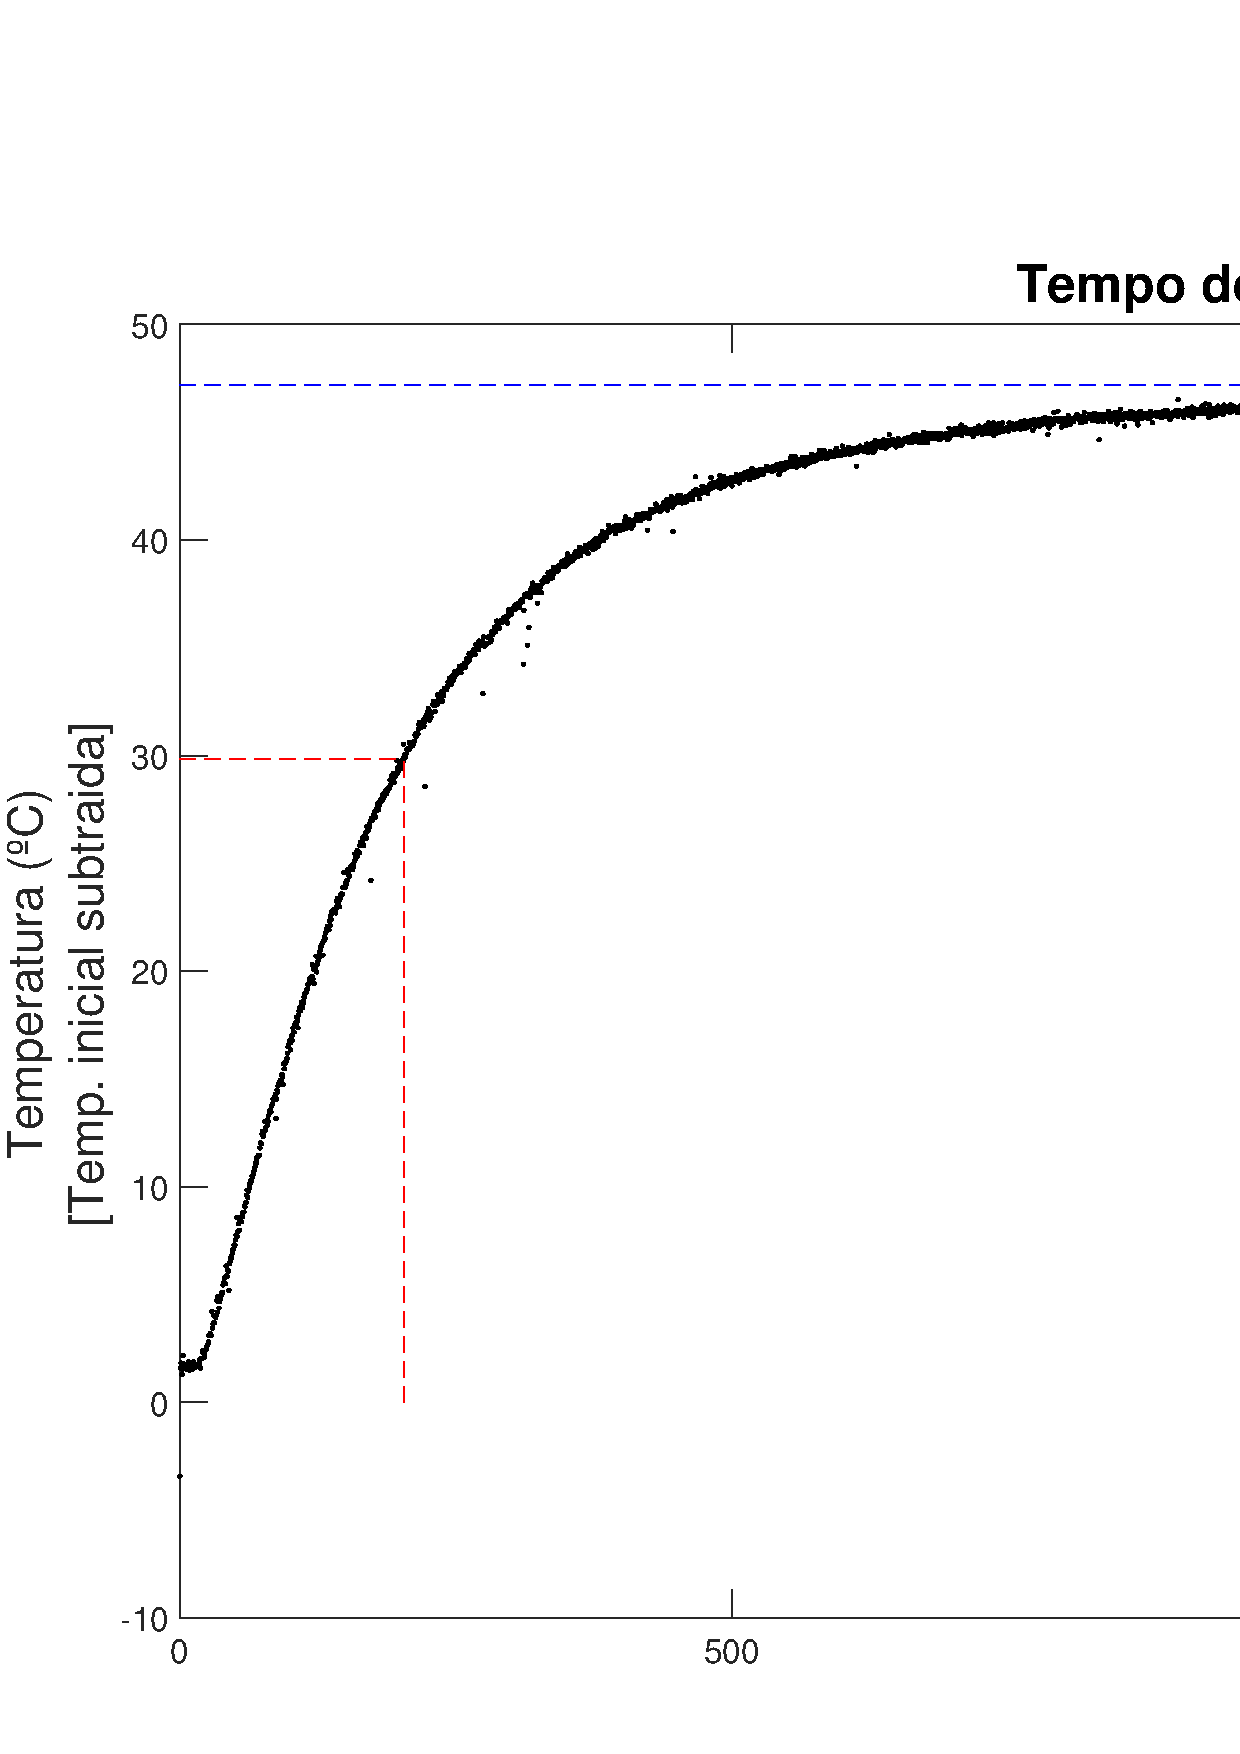
\includegraphics[width=0.85\textwidth]{./5_images/RiseTime-TempSensor1.png} 
		\label{fig:rise_time_sensor1}
	\end{center}
	\centering
	\makebox[\width]{Fonte: \citeonline{Prata2019}} 
\end{figure}

\begin{figure}[h]
	\caption{Tempo de subida - Sensor de Temperatura 1}
	\begin{center}
		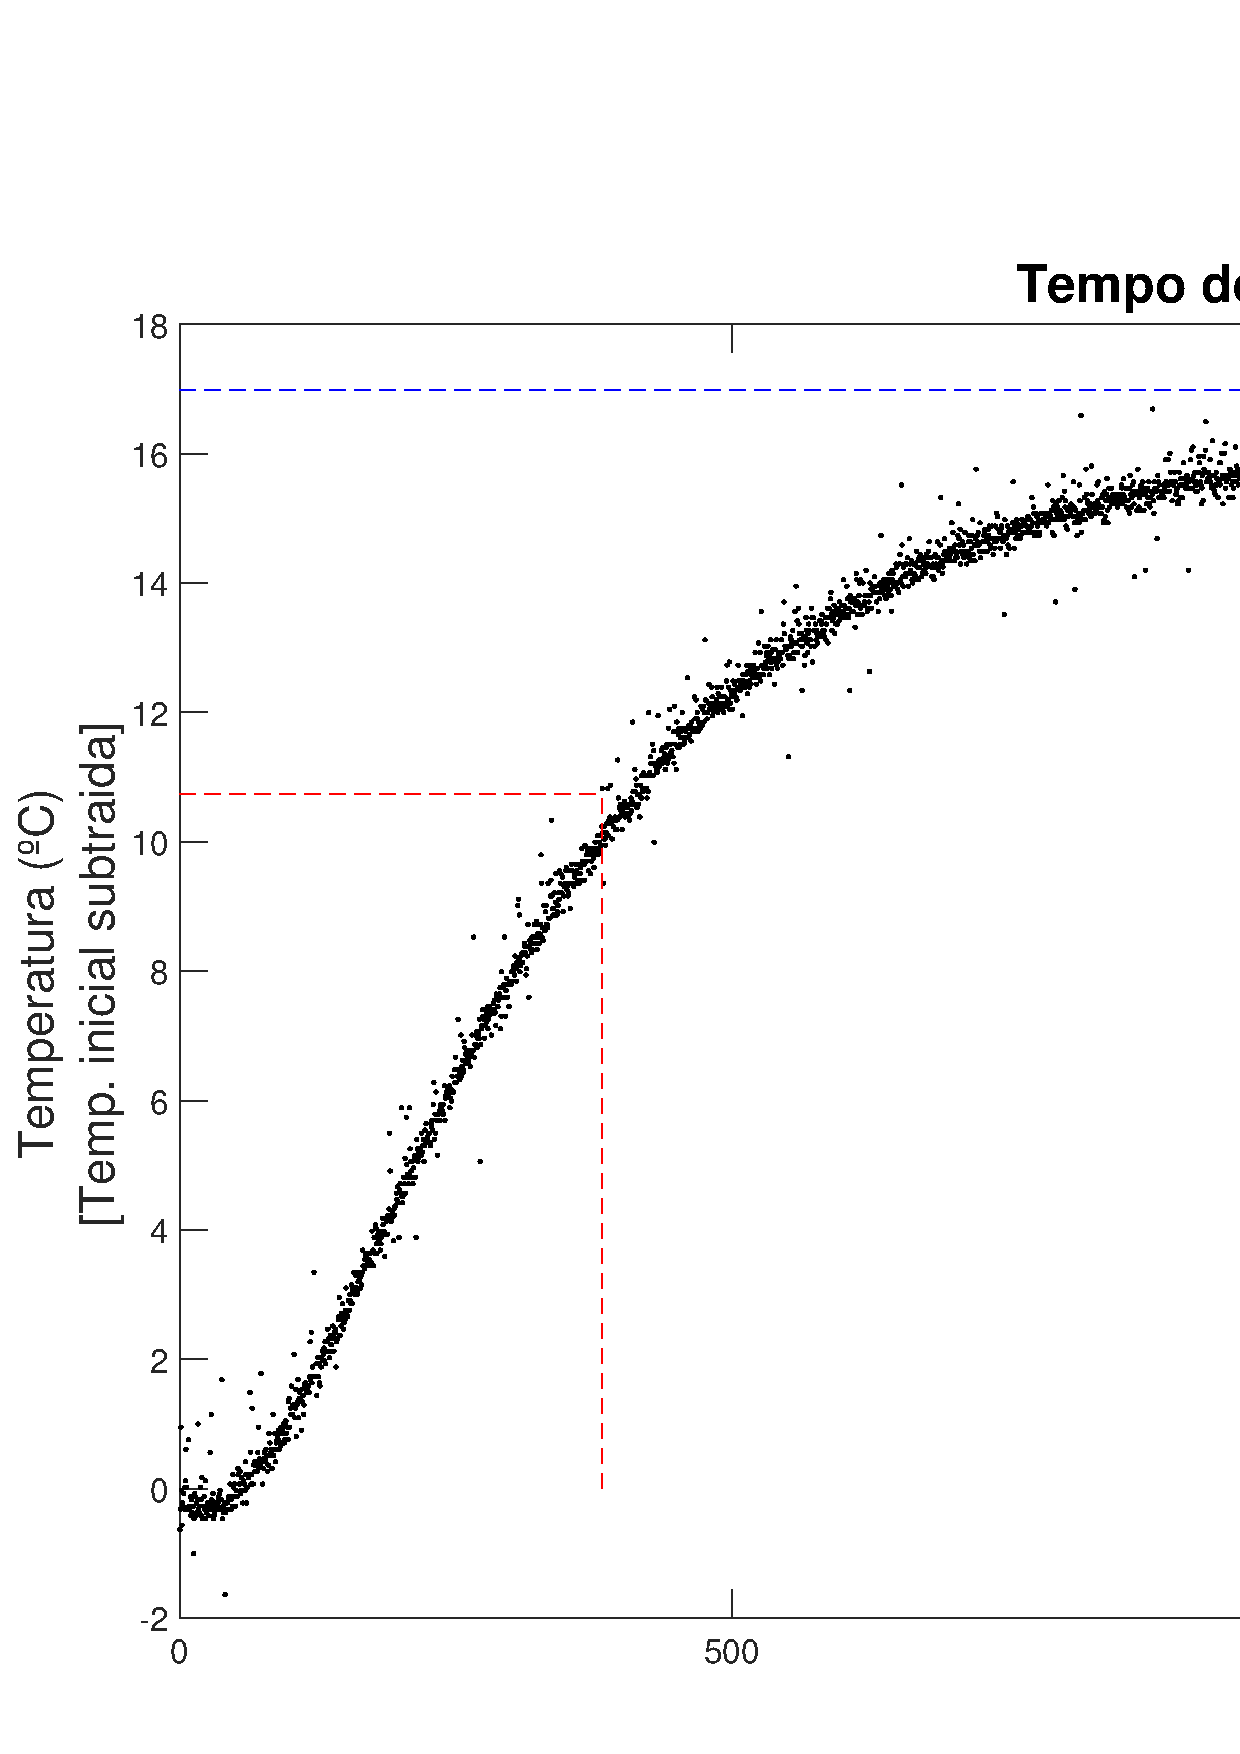
\includegraphics[width=0.85\textwidth]{./5_images/RiseTime-TempSensor2.png} 
		\label{fig:rise_time_sensor2}
	\end{center}
	\centering
	\makebox[\width]{Fonte: \citeonline{Prata2019}} 
\end{figure}

As \cref{fig:rise_time_sensor1,fig:rise_time_sensor2} mostram a resposta em malha aberta dos Sensores de
Temperatura 1 e 2, respectivamente, a uma entrada degrau no Aquecedor 1. Este ensaio foi realizado com
um período de amostragem de 0,5s, e com ele foi possível observar um tempo de subida $\tau_1 = 209s$ para
o Sensor 1 e $\tau_2 = 306s$ para o Sensor 2.
% TODO: Fazer mais ensaios com step 0 -> 50
% TODO: Recortar as imagens para remover bordas brancas

Seguindo a regra prática de \citeonline{Aguirre2015} onde $T_s$ deve ser entre 5 e 10 vezes maior que a
maior frequência desejada, então temos que $20.9s > T_s > 41.8s$.

Para os ensaios realizados neste trabalho, optou-se pela maior frequência de amostragem possível, como
mostrado na \cref{eq:sampling_time}.

\begin{equation}
	\label{eq:sampling_time}
	T_s = 20.9s
\end{equation}

Outra técnica também descrita por \citeonline{Aguirre2015} para a escolha da frequência de amostragem,
apesar de não ter sido escolhida, também foi testada e é descrita em maiores detalhes no
\cref{ch:sampling_time_using_autocorrelation}.

% TODO: Criar 'subsubsections' com os dois itens restantes abaixo.
\begin{itemize}
    % \item Período de amostragem: três regras práticas auxiliam na definição deste período: usar um tempo
    %     de amostragem de aproximadamente 1/10 da maior constante de tempo \apud{Gustavsson1975}{Ballin2008};
    %     10\% do tempo de acomodação de uma resposta degrau \cite{Ballin2008}; ou escolher uma frequência de amostragem
    %     de 5 a 10 vezes maior do que a maior frequência de interesse contida nos dados. \cite{Aguirre2015}.
    
    \item Sinais de excitação: a escolha dos sinais de entrada pode ter grande impacto nos dados coletados,
        pois determinarão o ponto de operação do sistema e quais das suas características serão excitadas
        durante o experimento \cite{Aguirre2015}.
        Diversos tipos distintos de sinais podem ser utilizados. Entre os mais utilizados destacam-se:
        impulsivo; degrau; \acrshort{prbs} - Sinal Binário Pseudo-Aleatório (do inglês, \acrlong{prbs});
        \acrshort{arma} - Média Móvel Auto-Regressiva (do inglês, \acrlong{arma});
        \acrshort{gbn} - Ruido Binário Generalizado (do inglês, \acrlong{gbn}); soma de senóides e etc.
        \cite{Aguirre2015}
    
    \item Duração do experimento: a duração do experimento, segundo \citeonline{Garcia2005}, deveria ser
        a maior possível, uma vez que a variância das estimativas é proporcional ao inverso da duração do
        experimento, porém sob o ponto de vista prático e experimental, a duração do experimento deveria ser
        a menor possível para a obtenção de um modelo aceitável, pois ao longo do experimento o processo
        estará sujeito a perturbações extras que podem impactar na operação da planta, na qualidade dos
        produtos ou até na segurança do processo.
\end{itemize}

% .....................................................................................................
% ............................................ Subsection .............................................
% .....................................................................................................
\subsection{Escolha da representação matemática}
\label{subsec:escolha_da_representacao_matematica}

Existem diversas representações matemáticas distintas para modelos lineares, sendo que, segundo
\citeonline{Aguirre2015}, a mais utilizada é a função de transferência, porém \citeonline{Wang2009}
destaca que nos últimos anos tem se observado um aumento na popularidade dos modelos de espaço de
estados para desenvolvimento de controle preditivo. Para \citeonline{Aguirre2015} é importante ainda
salientar o modelo \acrshort{ar} (\acrlong{ar}), o modelo \acrshort{arx} (\acrlong{arx}) e
o modelo \acrshort{armax} (\acrlong{armax}).

\begin{citacao}
    \text{[...]} quando se trata da modelagem obtida por meios fenomenológicos é comum que se adote a base de
    tempo contínuo, em virtude de a maioria das leis da física serem expressas nesse tempo. Por sua vez,
    quando se trata de identificação de sistemas por processos experimentais, trabalha-se com amostras
    de dados coletados a cada intervalo de tempo, nesses casos usualmente adota-se o tempo discreto.
    \apud{Garcia2005}{Favaro2012}
\end{citacao}

% .....................................................................................................
% ............................................ Subsection .............................................
% .....................................................................................................
\subsection{Determinação da estrutura do modelos}
\label{subsec:determinacao_da_estrutura_do_modelo}

Determinar a ordem de um modelo é um dos aspectos mais importantes na determinação de sua estrutura,
uma vez que, caso sua ordem seja muito menor do que a ordem efetiva do sistema real, o modelo não
refletirá a completamente sua complexidade estrutural. Analogamente, escolher um modelo que a ordem
seja muito maior do que a necessária, provavelmente causará uma estimação de parâmetros mal condicionada.
\cite{Aguirre2015}

% .....................................................................................................
% ............................................ Subsection .............................................
% .....................................................................................................
\subsection{Estimação de parâmetros}
\label{subsec:estimacao_de_parametros}

A estimação de parâmetros, segundo \apudonline{Eykhoff1974}{Favaro2012} é a determinação experimental
de valores de parâmetros que governam a dinâmica e/ou o comportamento não-linear, assumindo que a
estrutura do modelo seja conhecida.

Essa etapa começa com a escolha do algoritmo a ser utilizado \cite{Aguirre2015}. Dentre eles, os
mais amplamente empregados na literatura são: método da análise de frequência; método da resposta
transitória e método dos mínimos quadrados \cite{Favaro2012}.

% .....................................................................................................
% ............................................ Subsection .............................................
% .....................................................................................................
\subsection{Validação do modelo}
\label{subsec:validacao_do_modelo}

Em problemas de validação, a questão é tentar determinar se um dado modelo é válido ou não e para isso,
deve-se simulá-lo sem qualquer ajuste adicional e compará-lo a dados medidos em testes diferentes daquele
usado no desenvolvimento da sintonia do mesmo. Ao se obter um conjunto de modelos, deve-se verificar se
eles incorporaram as características de interesse do sistema original \cite{Aguirre2015}.

\citeonline{Aguirre2015} em seu livro apresenta diversas ferramentas para auxiliar na validação dos modelos.

% =====================================================================================================
% ============================================= Section ===============================================
% =====================================================================================================
\section{Desenvolvimento do controlador}
\label{sec:desenvolvimento_do_controlador}

Através das \cref{eq:tclab_modelo_siso,eq:tclab_modelo_mimo_a,eq:tclab_modelo_mimo_b}
e também do modelo experimental que será obtido da planta piloto, utilizaremos a representação de
espaço de estados para a construção do modelo que irá compor os controladores.

Serão utilizadas duas abordagens principais:

\begin{itemize}
    \item \textbf{Utilização apenas de linguagens de programação, sem o auxílio de ferramentas de desenvolvimento
        \acrshort{mpc}}: esta abordagem tem como meta aplicar o controle \acrshort{mpc} através dos algoritmos
        descritos nas obras de \citeonline{Wang2009}, \citeonline{Rawlings2015}, \citeonline{Rossiter2003},
        entre outros, com a finalidade de detalhar cada etapa dos cálculos realizados pelo controlador
        visando cumprir os seguintes objetivos descritos na seção \ref{sec:objetivos}: estudo do algoritmo do
        controle \acrshort{mpc}; comparação entre a implementação em duas ou mais plataformas e compilação
        de material teórico e experimental sobre \acrshort{mpc}.
    \item \textbf{Utilização de ferramentas de desenvolvimento \acrshort{mpc}}: esta abordagem visa utilizar
        ferramentas consolidadas de mercado para o desenvolvimento de controlador \acrshort{mpc}, como o
        \textit{Model Predictive Control Toolbox}, disponível no \acrshort{matlab} para poder realizar
        a comparação entre o desempenho de um controlador \acrshort{mpc} em comparação a um controlador
        \acrshort{pid}, como também foi proposto nos objetivos da seção \ref{sec:objetivos}.
\end{itemize}

% PARTE RESULTADOS E DISCUSSAO
\part{Resultados e discussão}

\chapter{Plano de Trabalho e Cronograma}
\label{ch:plano_de_trabalho_e_cronograma}

% TODO: alguma introdução

\section{Plano de Trabalho}
\label{sec:plano_de_trabalho}

% TODO: plano de trablhao

\section{Cronograma}
\label{sec:cronograma}

% TODO: Cronograma


% ELEMENTOS PÓS-TEXTUAIS
\postextual

% Referências bibliográficas
\bibliography{./3_posText/library}

% Glossário
% Consulte o manual da classe abntex2 para orientações sobre o glossário.
% % ----------------------------------------------------------
% Glossário
% ----------------------------------------------------------

% ---
% Define nome e preâmbulo do glossário
% ---
\phantompart
%\renewcommand{\glossaryname}{Glossário}  A opção babel do glossaries faz a tradução.
\renewcommand{\glossarypreamble}{Esta é a descrição do glossário. Experimente
visualizar outros estilos de glossários, como o \texttt{altlisthypergroup},
por exemplo.\\
\\}

% ---
% Traduções para o ambiente glossaries
% ---  
% A opção babel do glossaries faz a tradução.

%\providetranslation{Glossary}{Glossário}
%\providetranslation{Acronyms}{Siglas}
%\providetranslation{Notation (glossaries)}{Notação}
%\providetranslation{Description (glossaries)}{Descrição}
%\providetranslation{Symbol (glossaries)}{Símbolo}
%\providetranslation{Page List (glossaries)}{Lista de Páginas}
%\providetranslation{Symbols (glossaries)}{Símbolos}
%\providetranslation{Numbers (glossaries)}{Números} 
% ---

% ---
% Estilo de glossário
% ---
% \setglossarystyle{index}
% \setglossarystyle{altlisthypergroup}
 \setglossarystyle{tree}  % Já selecionado no arquivo .sty 


% ---
% Imprime o glossário
% ---
\cleardoublepage
\phantomsection
\addcontentsline{toc}{chapter}{\glossaryname}
\printglossaries % imprime todas as entradas

\imprimirglossario  % não imprime acronimos (siglas) e nem simbolos
% ---

% Apêndices
\begin{apendicesenv}

% Imprime uma página indicando o início dos apêndices
\partapendices

\chapter{Algum apêndice}

Incluir apêndice

\end{apendicesenv}


% Anexos
\begin{anexosenv}

% Imprime uma página indicando o início dos anexos
\partanexos

\chapter{Documentação de funções}
\label{ch:documentacao_de_funcoes}

\section{\acrshort{matlab} - fmincon}
\label{sec:fmincon}

\includepdf[pages=-]{6_annex/fmincon.pdf}

\section{Python - scipy.optimize.minimize}
\label{sec:scipy_optimize_minimize}

\includepdf[pages=-]{6_annex/scipy_optimize_minimize.pdf}


\end{anexosenv}


% INDICE REMISSIVO
\phantompart
\printindex

\end{document}
